\chapter{Povezivanje razvojnog sustava i oblaka}

Oblak koju pruža platforma AWS i razvojni sustav ESP32-C3 dva su odvojena sustava koja moraju međusobno komunicirati i razmjenjivati podatke. Za ostvarenje njihove veze razvijena su dva programska rješenja:
\begin{enumerate}
	\item programska potpora za mikrokontroler, koja će omogućiti dinamičko povezivanje na Wi-Fi, spajanje na platformu AWS te slanje podataka u oblak,
	\item programska potpora za platformu AWS, koja će ostvariti umrežavanje uređaja u sustav, ažuriranje softvera na uređaju, pohranu primljenih podataka s uređaja te prikaz tih podataka u web aplikaciji. 
\end{enumerate} 

\section{Programska potpora za mikrokontroler}

Programska potpora za uređaj ESP32-C3 sastoji se od nekoliko komponenti:
\begin{itemize}
	\item dinamičko povezivanje na bežičnu mrežu,
	\item spajanje na platformu AWS,
	\item učitavanje novog softvera, 
	\item očitavanje senzorskih mjerenja, 
	\item slanje podataka u oblak protokolom MQTT.
\end{itemize}

Neke od navedenih komponenti izvršavaju se slijedno, dok se druge izvršavaju paralelno. Spajanje na Wi-Fi i povezivanje s platformom AWS ključni su koraci koji prethode bilo kakvom pokušaju slanja podataka u oblak. Isto tako, praćenje ažuriranja softvera i očitavanje mjerenja izvršavaju se paralelno u posebnim procesima budući da nisu sekvencijalni niti međusobno isključivi zadaci. U nastavku je pobliže opisan svaki navedeni segment programske potpore. 

\subsection{Dinamičko povezivanje mikrokontrolera na Wi-Fi}

Radni okvir ESP-IDF nudi dinamičko spajanje na Wi-Fi mrežu pomoću zasebne komponente. Ovaj se postupak naziva provizioniranje \engl{provisioning}. Ova komponenta pruža aplikacijska programska sučelja \engl{Application Programming Interface - API} koja kontroliraju pružanje usluge za primanje i konfiguriranje Wi-Fi vjerodajnica putem sigurnih komunikacijskih protokola. Sigurnosni protokoli definirani su u komponenti protokolne komunikacije \engl{protocomm} koja upravlja sigurnim sjednicama \engl{sessions} i pruža radni okvir za višestruki prijenos podataka. Također je moguće direktno koristiti sloj protokolne komunikacije radi implementacije specifične za aplikaciju \cite{unified_provisioning}.

Sloj protokolne komunikacije interno koristi mehanizam protokolnih međuspremnika \engl{protocol buffers - protobuf} za sigurno uspostavljanje sjednice. Protokolni međuspremnici namijenjeni su za serijalizaciju strukturiranih podataka neovisno o programskom jeziku i platformi. Koristan je pri izradi programa i sustava koji međusobno komuniciraju putem mreže zbog kompaktnosti i niske latencije \cite{what_is_protobuf}.

Sloj protokolne komunikacije pruža radni okvir za različite načine komunikacije:
\begin{enumerate}
	\item protokol BLE,
	\item Wi-Fi (SoftAP u kombinaciji s HTTP serverom).
\end{enumerate}

Pružajući korisnicima okvir za ostvarivanje usluge dinamičkog povezivanja u mrežu, neovisno o načinu komunikacije, ovakva vrsta podrške naziva se unificirano provizioniranje \engl{unified provisioning}. Ovakav način prijave uređaja na mrežu zahtijeva interakciju korisnika putem vanjskog uređaja za slanje vjerodajnica na mikrokontroler. Tvrtka \textit{Espressif} pruža jednostavna mobilna rješenja koja se mogu koristiti gotova ili pak uklopiti u vlastitu mobilnu aplikaciju. Na slici \ref{fig:unified_provisioning} prikazana je arhitektura usluge.

\begin{figure}[ht]
	\centering
	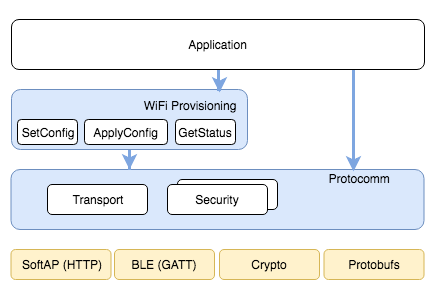
\includegraphics[scale=0.8]{imgs/unified_provisioning}
	\caption{Arhitektura unificiranog provizioniranja \cite{unified_provisioning}}
	\label{fig:unified_provisioning}
\end{figure}

Kao što je ranije opisano, arhitektura je bazirana na sloju protokolne komunikacije koji je odgovoran za prijenos podataka i sigurnost. Služi za jednostavne povratne pozive aplikaciji \engl{callbacks} i dobivanje Wi-Fi statusa. Sama aplikacija ima kontrolu nad implementacijom povratnih poziva. 

Aplikacija stvara instancu protokolne komunikacije koja se preslikava na određeni prijenosni protokol i sigurnosnu shemu. Svaki prijenos podataka u sloju protokolne komunikacije ima koncept krajnje točke \engl{endpoint} koji odgovara logičkom komunikacijskom kanalu za određenu vrstu informacija. Primjerice, sigurnosno rukovanje \engl{handshake} odvija se na različitoj krajnjoj točki u odnosu na točku za Wi-Fi konfiguraciju. Svaka se krajnja točka identificira nizom znakova i mijenja se ovisno o internom prikazu krajnje točke. U slučaju prijenosa pomoću Wi-Fi veze odnosno SoftAP funkcionalnosti, krajnja točka prikazuje se kao URI, dok u slučaju prijenosa podataka putem protokola BLE odgovara GATT karakteristici sa specifičnim identifikatorom. 

Oglašavanje i otkrivanje uređaja prepušteno je aplikaciji i ovisno o odabranom protokolu, vanjske aplikacije mogu odabrati odgovarajuću metodu za oglašavanje i otkrivanje. Za Wi-Fi prijenos obično se koristi ime mreže pristupne točke. Za prijenos putem protokola BLE može se koristiti ime samog uređaja. 

Kao što je opisano, podržano je korištenje protokola BLE kao i Wi-Fi usluge za prijenos vjerodajnica. Pri odabiru prijenosnog kanala za spajanje uređaja u mrežu, potrebno je razmotriti nekoliko točaka. Za početak, prijenos temeljen na protokolu BLE prednost održavanja netaknutog komunikacijskog kanala između uređaja i klijenta tijekom prijenosa podataka, što osigurava pouzdanu povratnu informaciju. S druge strane, prijenos putem Bluetootha troši oko 110 KB memorije tijekom rada, što je na uređajima niskih resursa velika potrošnja. Korisno je što se korištena memorija može vratiti na hrpu \engl{heap} po završetku umrežavanja uređaja ukoliko se BLE funkcionalnosti više ne koriste. Prijenos temeljen na Wi-Fi mreži, odnosno SoftAP funkcionalnosti, vrlo je interoperabilan i ne troši dodatnu memoriju. Međutim, mikrokontroler koristi isti radio za emitiranje pristupne točke i za spajanje na željenu mrežu. Budući da se te akcije mogu odvijati na različitim kanalima, postoji mogućnost da se ažuriranja statusa veze ne dostave na mobilni uređaj. Također, mobilni se uređaj mora odspojiti s izvorne Wi-Fi mreže radi privremenog spajanja na pristupnu točku mikrokontrolera. Uređaj će se spojiti na izvornu mrežu tak kada mikrokontroler ugasi pristupnu točku \cite{unified_provisioning}. 

Za razvoj predloženog rješenja korišteno je slanje vjerodajnica pomoću Wi-Fi mreže, odnosno privremene pristupne točke. Kao što je ranije opisano, protokol BLE troši značajnu količinu \textit{heap} memorije, a razvojni sustav ESP32-C3 nema dovoljno radne memorije koja bi pokrila prijavu u mrežu uz ostale radne procese. Mikrokontroler najprije stvori privremenu pristupnu točku na koju se mobilni uređaj spaja pomoću mobilne aplikacije. Zatim, nakon skeniranja dostupnih Wi-Fi mreža u blizini, u mobilnoj aplikaciji odabire se željena mreža i unese lozinka. Vjerodajnice se zatim pošalju putem Wi-Fi mreže, i mobilni uređaj može se odspojiti s privremene pristupne točke. Vjerodajnice se pohrane u memoriju tipa NVS \engl{non-volatile storage} koja ne zahtijeva konstantno napajanje kako bi se zadržala na uređaju. Ovime je omogućeno povezivanje uređaja u sustav čak i kada dođe do prekida napajanja \cite{what_is_nvs}. Memorija tipa NVS može se jedino programski obrisati, te bi u idealnom izvedbenom rješenju postojao vanjski gumb spojen na mikrokontroler koji bi pokretao brisanje te memorije i tako omogućio ponovno spajanje na željenu mrežu. Sljedeći programski isječak prikazuje inicijalizaciju memorije NVS, mrežnog sučelja te stvaranje pristupne točke.

\begin{lstlisting}[caption={Stvaranje pristupne točke}, language=c]
	/* Init NVS partition */
	esp_err_t ret = nvs_flash_init();
	/* Init TCP/IP */
	ESP_ERROR_CHECK(esp_netif_init());
	/* Init the event loop */
	ESP_ERROR_CHECK(esp_event_loop_create_default());
	wifi_event_group = xEventGroupCreate();
	/* Init Wi-Fi including netif with default config */
	esp_netif_create_default_wifi_sta();
	esp_netif_create_default_wifi_ap();
	wifi_prov_mgr_config_t config = {
		.scheme = wifi_prov_scheme_softap,
		.scheme_event_handler = WIFI_PROV_EVENT_HANDLER_NONE
	};
    /* Init provisioning manager with above config */
	ESP_ERROR_CHECK(wifi_prov_mgr_init(config));
	ESP_ERROR_CHECK(wifi_prov_mgr_start_provisioning(security, (const void *) sec_params, service_name, service_key));
	wifi_prov_print_qr(service_name, username, pop, PROV_TRANSPORT_SOFTAP, disp);
\end{lstlisting}

\subsubsection{LCD zaslon}

Za povezivanje mobilnog uređaja na privremenu pristupnu točku koju emitira razvojni sustav, potrebno je skenirati QR kod koji mikrokontroler generira. Budući da ESP32-C3 nema vlastito sučelje, na sustav je spojen zaslon OLED SSD1306 veličine 128×64 piksela. Uređaj sa zaslonom komunicira putem I2C sučelja, a za prikaz sadržaja na zaslonu korištena je biblioteka LVGL \engl{Light and Versatile Graphics Library}. To je grafička biblioteka otvorenog koda namijenjena izradi aplikacija s grafičkim korisničkim sučeljem \engl{Graphical User Interface - GUI} za ugradbene sustave. Pruža radni okvir s mnogim značajkama, temama i paletama boja. Isto tako, biblioteka troši vrlo malo resursa, što je čini pogodnom za uređaje poput razvojnog sustava ESP32-C3 \cite{lvgl}. Generiranje QR koda obavlja se pomoću biblioteke \textit{QR-Code-Generator} koja je prilagođena ESP32 uređajima. 

\begin{lstlisting}[caption={Generiranje QR koda iz pristupne točke}, language=c]
static void wifi_prov_print_qr(const char *name, const char *usrname, const char *pop, const char *transport, lv_disp_t *disp) {
	char payload[150] = {0};
    snprintf(payload, sizeof(payload), 	
    	"{\"ver\":\"%s\",\"name\":\"%s\",\"username\":\"%s\",\"pop\":\"%s\",\"transport\":\"%s\"}",
    	 PROV_QR_VERSION, name, usrname, pop, transport);
    esp_qrcode_config_t cfg = {
		.display_func = generate_qr_code_lcd, 
		.max_qrcode_version = 10, 
		.qrcode_ecc_level = ESP_QRCODE_ECC_LOW
	};
	esp_qrcode_generate(&cfg, payload);
}
\end{lstlisting}

Prethodna funkcija povezuje pristupnu točku s QR kodom. Podaci o samoj pristupnoj točki učitaju se u privremenu varijablu, čiji se sadržaj prosljeđuje biblioteci za generiranje QR koda. Dobiveni se podaci zatim prosljeđuju funkciji za prikaz koda na zaslonu. QR kod prikazuje se na zaslonu piksel po piksel, skalirajući veličinu QR koda na temelju širine i duljine samog zaslona. 

\begin{lstlisting}[caption={Funkcija za prikaz QR koda na zaslonu}, language=c]
void generate_qr_code_lcd(esp_qrcode_handle_t qrcode)
{
	ESP_LOGI(TAG, "%s", "Started generate_qr_code_lcd...");
	
	int size = qrcodegen_getSize(qrcode);
	
	// Calculate the scale factor
	int scale = (int)fmin(EXAMPLE_LCD_H_RES / size, EXAMPLE_LCD_V_RES / size);
	
	// Calculate horizontal shift
	int shift_x = (EXAMPLE_LCD_H_RES - size * scale)/2;
	
	// Calculate vertical shift
	int shift_y = (EXAMPLE_LCD_V_RES - size * scale)/2;
	
	if (lvgl_port_lock(0)) {
		lv_obj_t *screen = lv_scr_act();
		lv_obj_clean(screen); // Clear the screen to ensure it's dark
		
		// Create a canvas object
		lv_obj_t *canvas = lv_canvas_create(screen);
		static lv_color_t cbuf[LV_CANVAS_BUF_SIZE_TRUE_COLOR(EXAMPLE_LCD_H_RES, EXAMPLE_LCD_V_RES)];
		lv_canvas_set_buffer(canvas, cbuf, EXAMPLE_LCD_H_RES, EXAMPLE_LCD_V_RES, LV_IMG_CF_TRUE_COLOR);
		lv_canvas_fill_bg(canvas, lv_color_white(), LV_OPA_COVER);
		
		// Draw the QR code on the canvas
		for (uint8_t y = 0; y < size; y++) {
			for (uint8_t x = 0; x < size; x++) {
				if (qrcodegen_getModule(qrcode, x, y)) {
					for (int dy = 0; dy < scale; dy++) {
						for (int dx = 0; dx < scale; dx++) {
							lv_canvas_set_px(canvas, shift_x + x * scale + dx, shift_y + y * scale + dy, lv_color_black());
						}
					}
				}
			}
		}
		
		// Release the mutex
		lvgl_port_unlock();
	}
}
\end{lstlisting}

Na slikama \ref{fig:esp_softap_app1} i \ref{fig:esp_softap_app2} prikazana je mobilna aplikacija te trenutak nakon skeniranja QR koda. Mobilni uređaj zahtijeva spajanje na privremenu pristupnu točku, a iduća slika prikazuje dostupne Wi-Fi mreže u blizini mobilnog uređaja, ujedno i mikrokontrolera, na koje se razvojni sustav može spojiti. Odabirom jedne od mreža i unosom lozinke vjerodajnice se šalju na razvojni sustav.

\begin{figure}[ht]
	\begin{minipage}[t]{0.3\textwidth}
		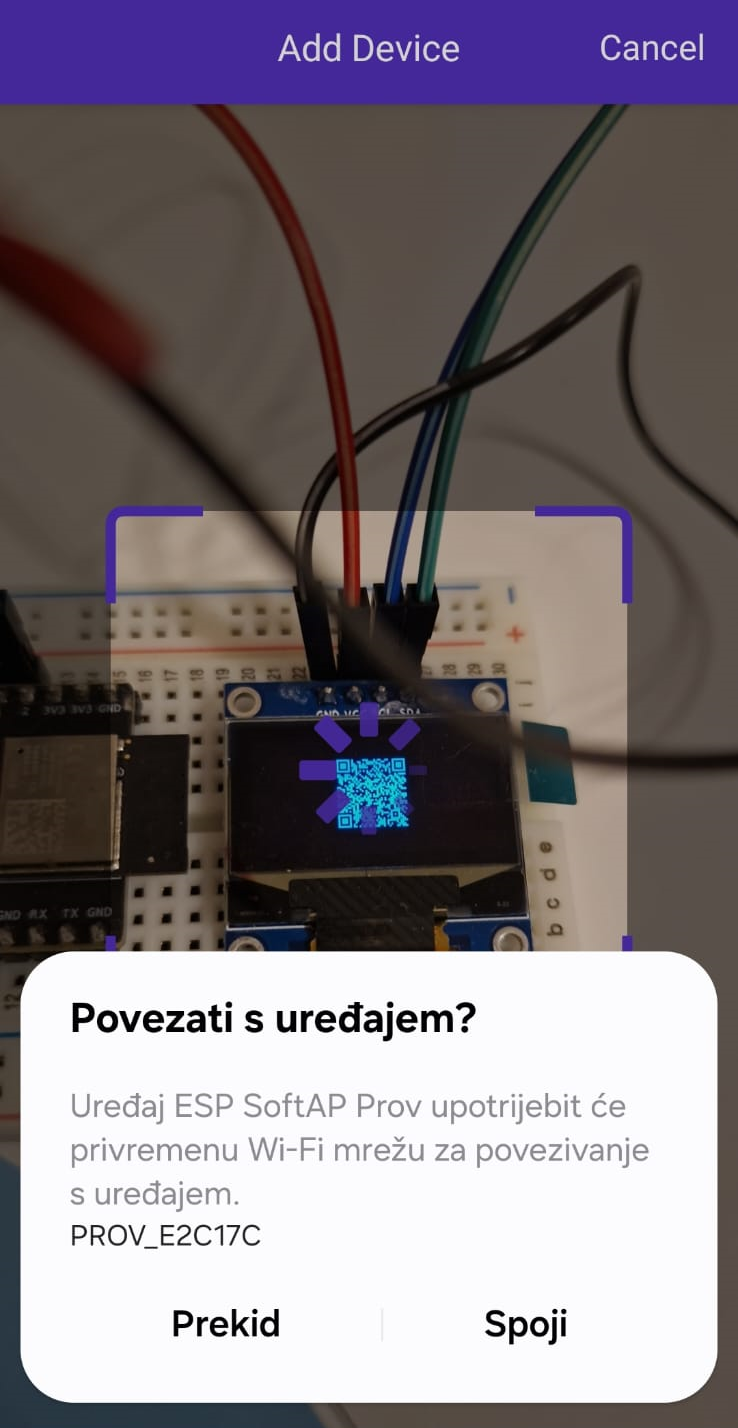
\includegraphics[width=\linewidth]{imgs/esp_softap_app1}
		\caption{Obavijest nakon skeniranja QR koda}
		\label{fig:esp_softap_app1}
	\end{minipage}
	\hspace*{\fill}
	\begin{minipage}[t]{0.3\textwidth}
		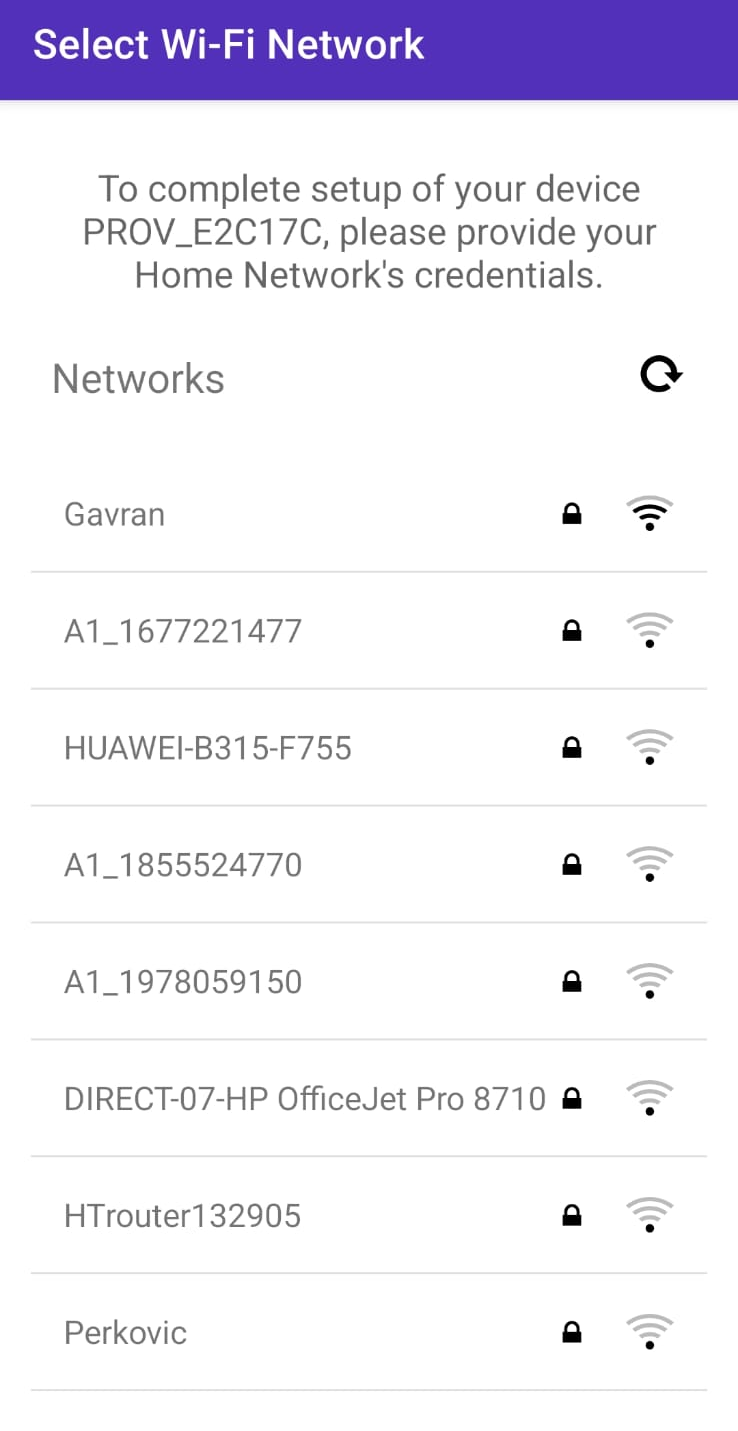
\includegraphics[width=\linewidth]{imgs/esp_softap_app2}
		\caption{Odabir dostupne Wi-Fi mreže u blizini}
		\label{fig:esp_softap_app2}
	\end{minipage}
\end{figure}

\subsection{Registracija u sustav AWS}

Nakon uspješnog povezivanja na Wi-Fi, sljedeći je korak registracija uređaja na platformu AWS. Korištena je biblioteka za AWS IoT Fleet Provisioning koja se održava u sklopu projekta otvorenog koda \textit{FreeRTOS} \cite{fleet_prov_sdk}. Biblioteka omogućuje mnoštvu odn. floti IoT uređaja registraciju i instalaciju jedinstvenih certifikata na platformu. Bibliotekom je moguće uređaje registrirati i pomoću autoriziranog korisnika, ali i certifikatima zahtjeva. Ova biblioteka ne ovisi o dodatnim bibliotekama osim standardne C biblioteke i stoga se može koristiti s bilo kojom bibliotekom za MQTT protokol.

Za potrebe ovog sustava odabrana je registracija pomoću certifikata zahtjeva. Na slici \ref{fig:fleet_provisioning_by_claim} prikazan je slijed događaja pri registraciji uređaja. Uređaj se najprije spaja na AWS certifikatom zahtjeva koji unaprijed postoji na mikrokontroleru te ostvaruje MQTT vezu. Zatim objavljuje praznu poruku na temu \textit{\$aws/certificates/create/json}, kojom zapravo podnosi zahtjev za kreiranjem vlastitog jedinstvenog certifikata. Usluga kreira traženi certifikat, pripadni ključ te generira značku vlasništva \engl{ownership token}, što sve skupa i objavljuje na temu \textit{\$aws/certificates/created/json/accepted}, na koju je uređaj pretplaćen. Razvojni sustav zatim sigurno pohranjuje dobivene vjerodajnice te objavljuje vlastite parametre i dobivenu značku na temu predloška za registraciju. Ako je kreirana, u sustavu AWS zatim se pokreće Lambda funkcija koja obavlja dodatne provjere nad dobivenim parametrima i tako provjerava valjanost zahtjeva. Primjerice, uređaj pri slanju parametara šalje i hardversku tajnu, koja se može zatim provjeriti u bazi podataka sustava AWS s pohranjenim takvim tajnama i provjeriti valjanost te tajne. Pri uspješnoj provjeri, Lambda funkcija vraća \lstinline|{"allowProvisioning" : True}|, čime daje konačno zeleno svjetlo za registraciju. Usluga posljedično kreira stvar i pripadnu politiku definiranu u predlošku te aktivira novostvoreni certifikat. Objavljuje novu konfiguraciju specifičnu za uređaj na temu za potvrdu uspješne registracije. Razvojni se sustav, nakon primjene nove konfiguracije, povezuje jedinstvenim privatnim ključem te certifikatom na AWS. Ova se nova MQTT veza dalje koristi za komunikaciju i razmjenu podataka.

\begin{figure}[ht]
	\centering
	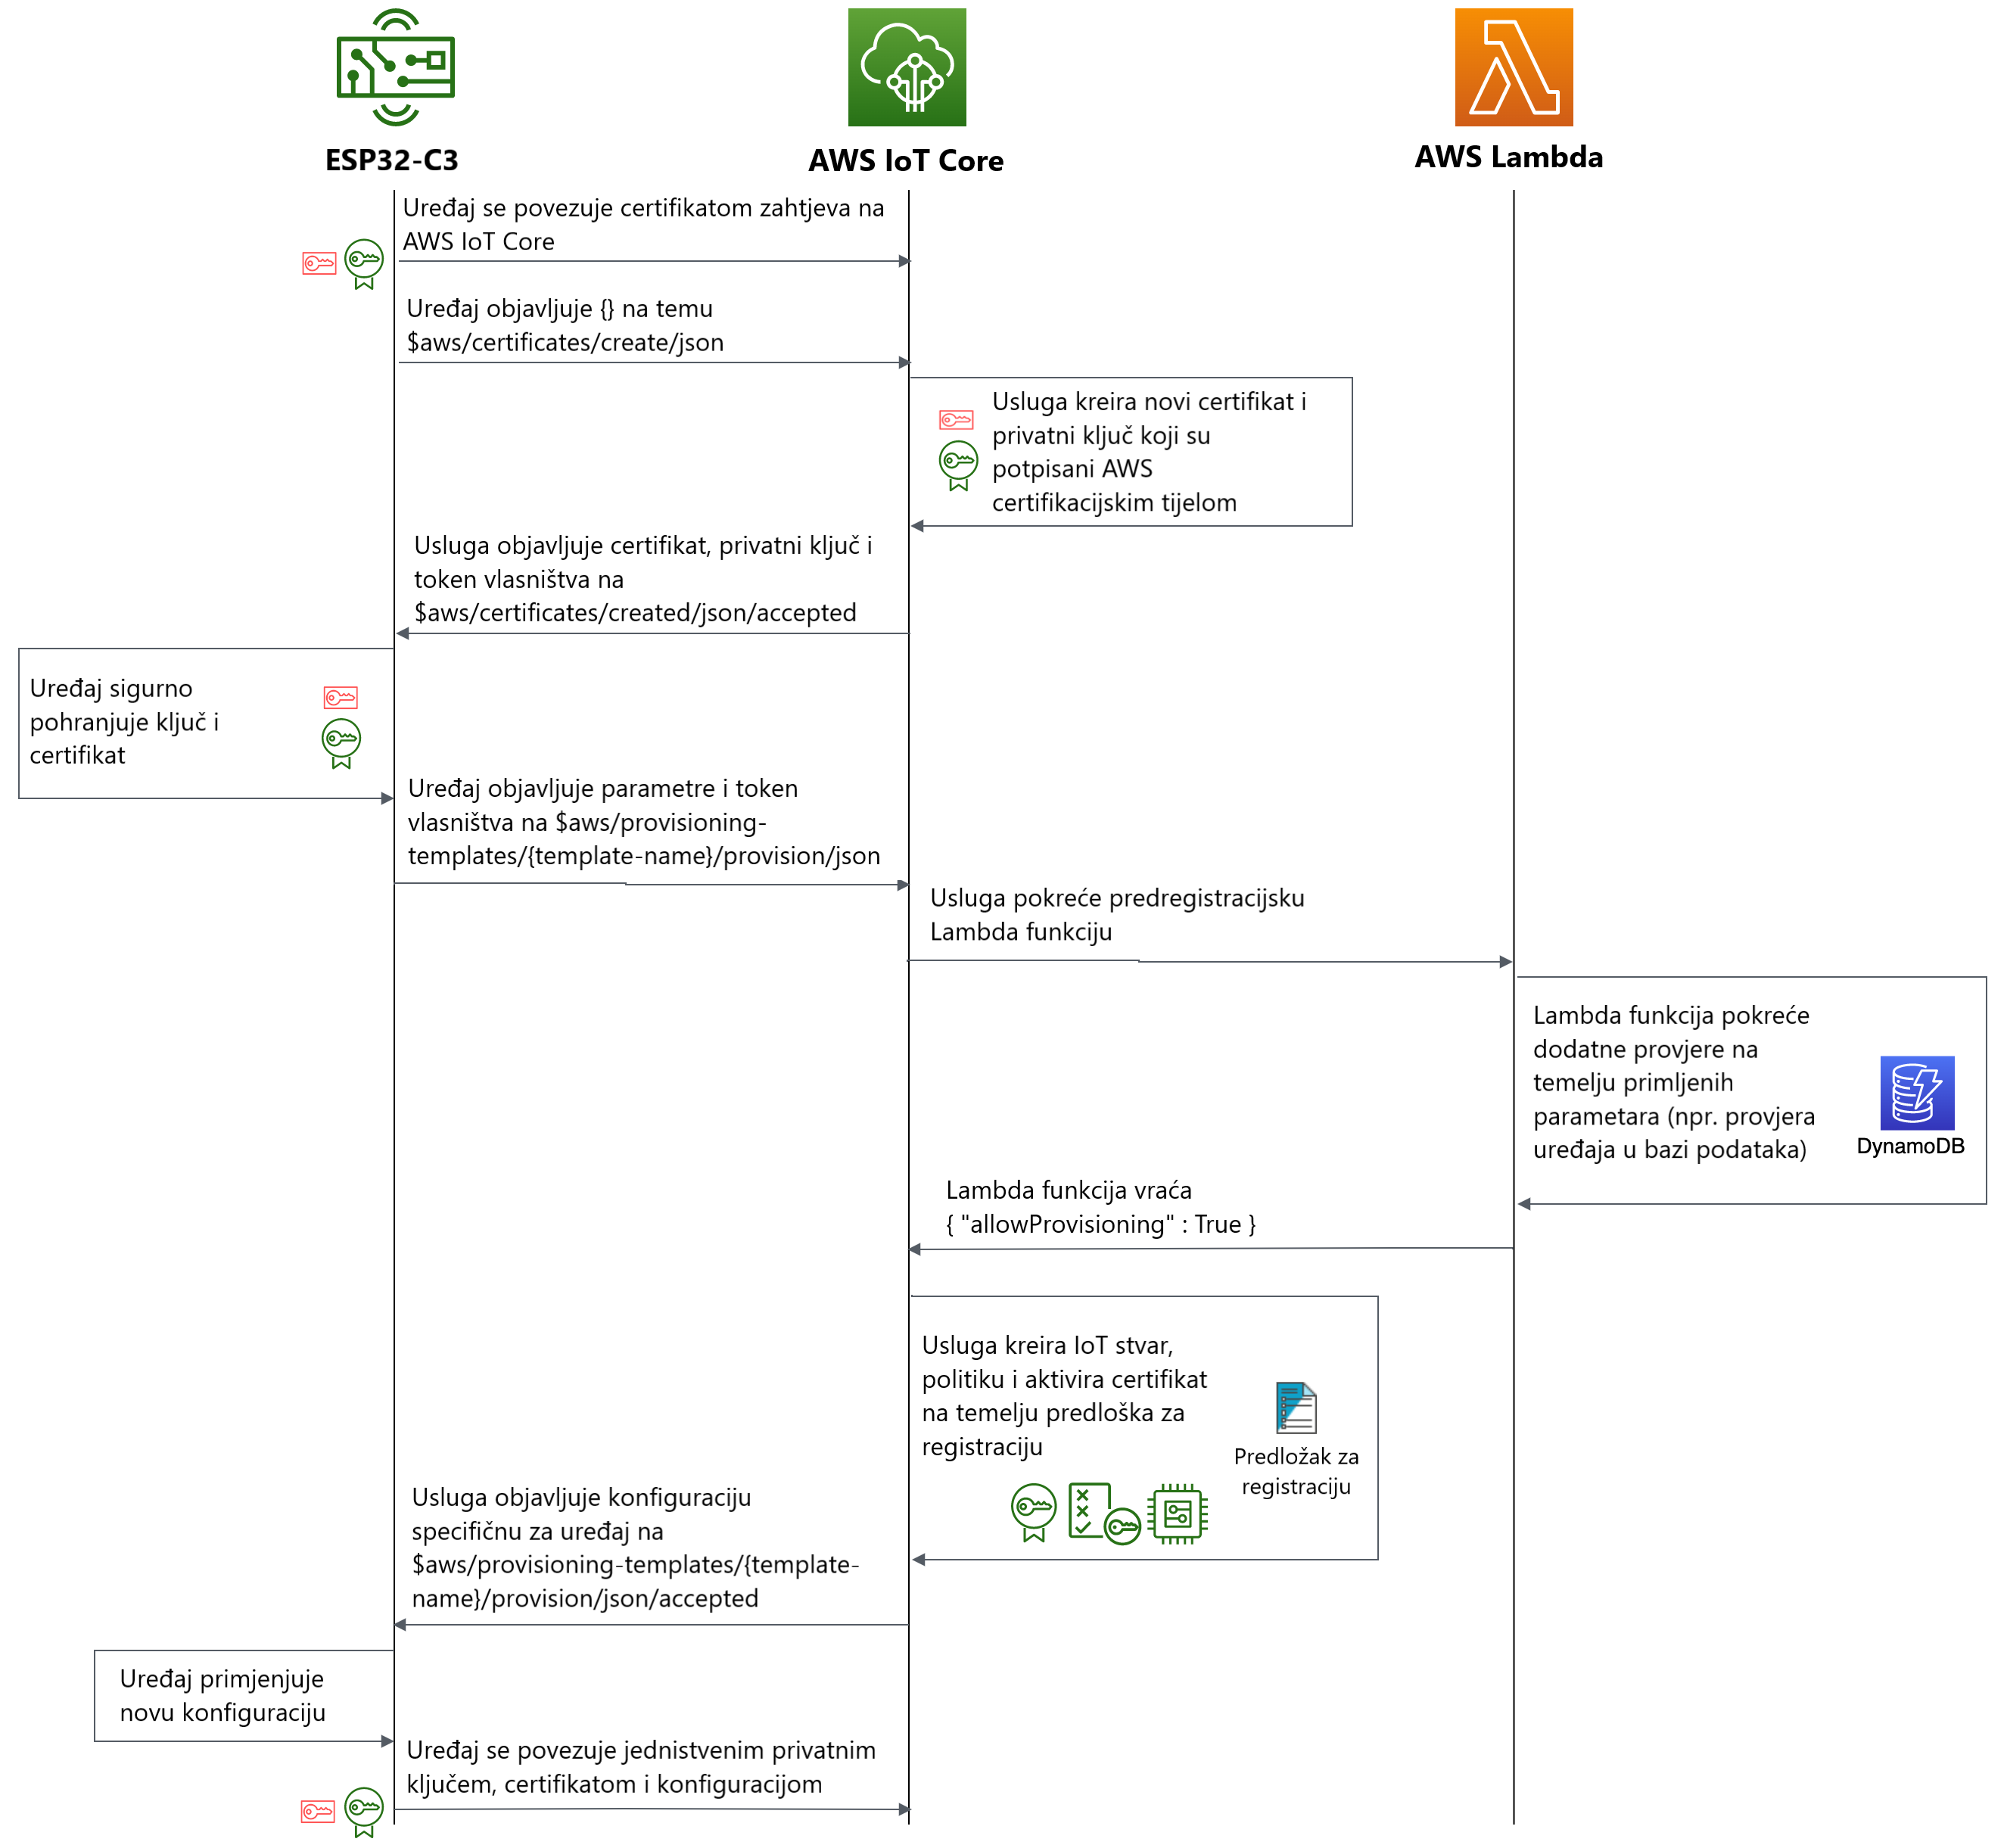
\includegraphics[scale=0.2]{imgs/fleet_provisioning_by_claim}
	\caption{Tok registracije uređaja certifikatom zahtjeva \cite{aws_docs}}
	\label{fig:fleet_provisioning_by_claim}
\end{figure}

Opisani tok ostvaren je uz pomoć ranije spomenute biblioteke, kao i knjižice \textit{coreMQTT} za komunikaciju putem protokola MQTT s API-jem platforme AWS. Za manipulaciju certifikatima i privatnim ključevima, korištena je biblioteka \textit{corePKCS11}. Ona koristi standard PKCS \#11 \engl{Public-key Certificate Standards}, što je široko korišten API za manipuliranje uobičajenim kriptografskim objektima. Funkcije koje navodi omogućuju aplikacijama korištenje, stvaranje, modificiranje i brisanje kriptografskih objekata, bez izlaganja tih objekata memoriji aplikacije. Primjerice, konkretna integracija s bibliotekom za registraciju uređaja koristi mali podskup PKCS \#11 API-ja za, između ostalog, pristup privatnom ključu potrebnom za stvaranje mrežne veze koja je autentificirana i zaštićena protokolom TLS bez da aplikacija ikada dođe u doticaj s ključem \cite{what_is_pkcs}. 

Sljedeći programski odsječak prikazuje uspostavu MQTT sjednice pomoću certifikata zahtjeva te podnošenje zahtjeva za novim certifikatom. U odsječku se također može primijetiti binarna serijalizacija podataka. Format CBOR \engl{Concise Binary Object Representation} Representation), za razliku od formata JSON, pretvara podatke u binarni oblik te ih tako šalje mrežom, što rezultira manjom latencijom i nosivošću \engl{payload} \cite{cbor}. Pri prijenosu velike količine podataka pri ograničenim resursima, poput u IoT sustava, ušteda na veličini poslanih podataka znatno utječe na efikasnost sustava. Isto tako, binaran je format prilagodljiv u odnosu na JSON, gdje mora postojati unaprijed definirana shema za primitak podataka.

\begin{lstlisting}[caption={Spajanje certifikatom zahtjeva i zahtjev za novim certifikatom}, language=c]
 LogInfo( ( "Establishing MQTT session with claim certificate..." ) );
 status = EstablishMqttSession( provisioningPublishCallback,
		*p11Session,
		pkcs11configLABEL_CLAIM_CERTIFICATE,
		pkcs11configLABEL_CLAIM_PRIVATE_KEY );
 status = subscribeToCsrResponseTopics();
 status = generateKeyAndCsr( *p11Session,
		pkcs11configLABEL_DEVICE_PRIVATE_KEY_FOR_TLS,
		pkcs11configLABEL_DEVICE_PUBLIC_KEY_FOR_TLS,
		csr,
		CSR_BUFFER_LENGTH,
		&csrLength );
/* Publish the CSR to CreateCertificatefromCsr API. */
 PublishToTopic( FP_CBOR_CREATE_CERT_PUBLISH_TOPIC,
		FP_CBOR_CREATE_CERT_PUBLISH_LENGTH,
		( char * ) payloadBuffer,
		payloadLength );
 status = waitForResponse();
\end{lstlisting}

\subsection{Očitavanje senzorskih mjerenja}

Razvijeni sustav, osim zaslona, sadrži dva senzora koja mjere stanja iz okoline: senzor za temperaturu i vlagu zraka te senzor za vlažnost tla. Mjerenja ovih senzora šalju se na platformu AWS i simuliraju stvarna poljoprivredna mjerenja. Mjerenje temperature i vlage zraka vrši se pomoću senzora DHT11, dok se vlažnost tla mjeri senzorom VMA303. 

\subsection{Slanje očitanih podataka protokolom MQTT}

\subsection{Ažuriranje softvera}

\section{Programska potpora za oblak}

Programska potpora za platformu AWS nije kod u standardnom smislu, no kako bi se uređaj i platforma uopće mogli komunicirati međusobno, potrebno je omogućiti povezivanje i komunikaciju na samoj platformi. Sva se komunikacija odvija u istoj AWS regiji. Zbog dostupnosti većine IoT usluga i relativne geografske bliskosti, korištena je regija \textit{eu-north-1} odnosno Stockholm, Švedska. 

Isto tako, važno je istaknuti kako se sve opisane radnje u sustavu AWS mogu izvršavati pomoću naredbenog retka platforme AWS \engl{Command-line interface - CLI}, no radi jednostavnosti i preglednosti, korišteno je korisničko sučelje platforme.

Programska potpora sastoji se od sljedećih segmenata:
\begin{itemize}
	\item omogućavanje dinamičke registracije uređaja,
	\item slanje novog softvera na uređaj,
	\item pristup zadnjem stanju uređaja nakon gubitka veze,
	\item obrada podataka dobivenih protokolom MQTT,
	\item pohrana podataka.
\end{itemize}

\subsection{Dinamička registracija uređaja}

Kao što je ranije opisano, u razvijenom sustavu koriste se certifikati zahtjeva za prvotno spajanje na platformu AWS, stoga je potrebno kreirati odgovarajući predložak za registraciju. Predložak također mora imati dodijeljenu politiku koja autorizira certifikat zahtjeva i ta se politika dodjeljuje generiranim certifikatima zahtjeva. Odabiru se politike koje omogućavaju točno onoliko koliko je potrebno za spajanje u sustav, a to su dopuštenja za MQTT komunikaciju i spajanje na AWS. Također, potrebno je odabrati koji su certifikati valjani kao zahtjev. Poželjno je i dodijeliti Lambda funkciju kao predregistracijsku provjeru dodatne valjanosti zahtjeva i poslanih parametara. Za razvijeni sustav nije kreirana Lambda funkcija, što znači da je svaki zahtjev automatski odobren. Isto tako, moguće je automatski pri registraciji uređaja kreirati i pripadnu stvar \engl{thing}, što je korisno za kasniju organizaciju i pregled certifikata. Svaka stvar može imati modularan naziv, ovisno o parametrima koji se pošalju. Za ovaj sustav postavljen je prefiks \textit{ESP32Thing\_} koji označava da su uređaji vrste ESP32, a ostatak naziva stvari ovisi o serijskom broju samog uređaja. To osigurava da svaki uređaj kreira jedinstvenu stvar u AWS-u. Moguće je odabrati i vrstu stvari \engl{thing type} koja će se automatski pridijeliti stvari, te u ovom slučaju kreirana je nova vrsta stvari naziva ESP32-C3. Stvarima se može dodijeliti i grupa, no u ovom sustavu nije bilo potrebe za kreiranjem dodatne grupe stvari budući da se povezuje samo jedna vrsta uređaja u sustav. Naposlijetku, potrebno je odabrati koje će se politike dodijeliti novogeneriranom jedinstvenom certifikatu, čime će uređaj dobiti pristup uslugama sustava AWS. Odabrane politike u ovom sustavu imaju sva dopuštenja radi lakše demonstracije funkcionalnosti. U nastavku se može vidjeti isječak kreiranog predloška, odnosno parametri stvari koja se kreira korištenjem predloška. U odsječku se isto tako može vidjeti funkcija za kreiranje imena stvari koja koristi predefinirani prefiks i serijski broj uređaja. 

\begin{lstlisting}[caption={Odjeljak \textit{stvar} u predlošku za registraciju}, language=json]
 "thing": {
	"Type": "AWS::IoT::Thing",
	"OverrideSettings": {
		"AttributePayload": "MERGE",
		"ThingGroups": "DO_NOTHING",
		"ThingTypeName": "REPLACE"
	},
	"Properties": {
		"AttributePayload": {},
		"ThingGroups": [],
		"ThingName": {
			"Fn::Join": [
			"",
			[ "ESP32Thing_", { "Ref": "SerialNumber" } ]
			]
		},
		"ThingTypeName": "ESP32-C3"
	}
 }
\end{lstlisting}

Na slici \ref{fig:policies} nalazi se popis politika koje su dodijeljene uređaju registriranom u sustav. Omogućene su sve politike, odnosno dodijeljene su sve dozvole koje uređaj može imati. Politika \textit{DevicePolicy} odnosi se na komunikaciju MQTT protokolom, \textit{DeviceShadowPolicy} na akcije vezane uz sjenu uređaja, \textit{JobPolicy} na izvršavanje i dohvat poslova te \textit{CertificatePolicy} dozvoljava povezivanje certifikatom. 

\begin{figure}[ht]
	\centering
	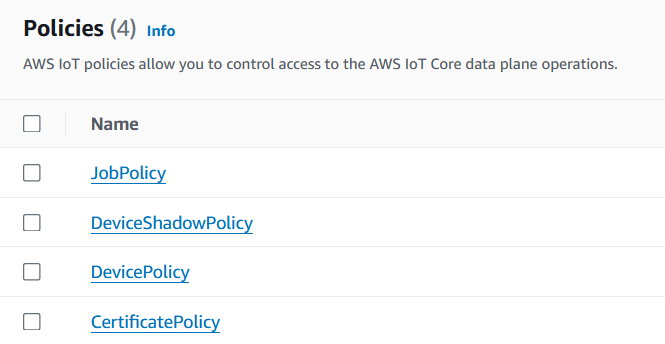
\includegraphics[scale=0.8]{imgs/policies}
	\caption{Popis politika dodijeljenih registriranom uređaju}
	\label{fig:policies}
\end{figure}
